\documentclass[12pt,a4paper]{report}
\usepackage{geometry}
\geometry{
	a4paper,
	total={170mm,257mm},
	left=20mm,
	top=20mm,
}\usepackage{graphicx}
\usepackage{tcolorbox}
\usepackage{mathtools}
\usepackage{tabu}
\tcbuselibrary{breakable}
\usepackage{listings}
\usepackage{xepersian}
\settextfont[Scale=1]{BNazanin}
\setlatintextfont[Scale=1]{Calibri}
\renewcommand{\baselinestretch}{1.5} 



\begin{document}
	\begin{titlepage}
		\centering
		
\includegraphics[width=0.45\textwidth]{Figures/logo}\par\vspace{1cm}
		{\scshape\LARGE  دانشکده مهندسی برق و کامپیوتر دانشگاه تهران \par}
		\vspace{1cm}
		{\scshape\Large  گزارش فصل 1: \lr{Inventory System}\par}
		\vspace{1.5cm}
		{\huge\bfseries امیرحسین مرادیان\par}
		\vspace{0.5cm}
		{\Large\itshape 810100467\par}
		\vfill
		\huge {استاد درس:}
		\par
		دکتر خونساری
		
		\vfill
		
		% Bottom of the page
		{\large \today\par}
	\end{titlepage}
	
	\pagebreak
	
	\section*{مقدمه}
شرکتی که یک محصول واحد را می‌فروشد می‌خواهد تصمیم بگیرد که چه آیتم‌هایی را باید در موجودی برای هر یک از $n$ ماه آینده در نظر بگیرد ($n$ یک پارامتر ورودی \lr{fixed} است.) زمان بین تقاضاها یک متغییر تصادفی با میانگین $0.1$ ماه است. سایز تقاضاها $D$ هست و یک متغییر تصادفی است. (مستقل از این‌که تقاضا کی اتفاق می‌افتد.) که $w.p$ احتمال را نشان می‌دهد:
\begin{align*}
	D=\begin{cases} 1& w.p. \frac{1}{6}\\
		2&w.p. \frac{1}{3}\\
		3& w.p. \frac{1}{3}\\
		4& w.p. \frac{1}{6}\end{cases}
\end{align*}
در ابتدای هر ماه، شرکت سطح موجودی را بررسی می‌کند و تصمیم می‌گیرد که برای سفارش از تأمین‌کننده آن‌چه آیتم‌هایی را درنظر بگیرد. اگر شرکت $z$ ایتم را سفارش بگیرد هزینه وارده برابر با $K+i*z$ خواهد بود که $K$ برابر با (هزینه راه‌اندازی) $32\$$ و $i$ برابربا  $3\$$ می‌باشد. اگر $z=0$ باشد هیچ هزینه‌ای نداریم. وقتی یک سفارش پذیرفته می‌شود، زمان لازم برای آن
\lr{delivery lag} یا \lr{lead time}
نامیده می‌شود و آن یک متغییر تصادفی با توزیع یکنواخت بین $0.5$ تا 1 ماه می‌باشد.

شرکت  از یک سیاست برای تصمیم‌گیری این‌که چه مقدار سفارش بگیرد به نام $(s,S)$  استفاده می‌کند:
\begin{align*}
	Z=\begin{cases}
		S-I& \mathrm{if}\; I<s\\
		0&\mathrm{if}\; I\geq s
	\end{cases}
\end{align*}
به گونه‌ای که $I$ سطح موجودی را در ابتدای هر ماه مشخص می‌کند.

وقتی یک تقاضا داریم، اگر سطح موجودی به اندازه تقاضا باشد، تقاضا به سرعت پاسخ داده می‌شود اما اگر تقاضا از سطح موجودی تجاوز کند، یک گزارش \lr{backlog} می‌فرستد و تقاضای مازاد در آینده تحویل داده می‌شود، (در این مورد سطح موجودی جدید برابر با سطح موجودی قدیم منهای اندازه تقاضا است که یک سطح منفی برای موجودی به‌وجود می‌آورد.) وقتی یک سفارش می‌رسد آن ابتدا سفارش‌های از قبل مانده (اگر موجود باشد) را پاسخ می‌دهد و باقیمانده را به سطح موجودی اضافه می‌کند.

ما فقط بر روی یک نوع از هزینه وارده بوسیله سیستم موجودی بحث می‌کنیم به نام هزینه سفارش. به هرحال بسیاری از سیستم‌های موجودی واقعی دو نوع هزینه اضافی دارند یکی هزینه  \lr{holding} و دیگری هزینه کمبود.

$I(t)$
سطح موجودی را در زمان $t$ مشخص می‌کند که مقدار مثبت، منفی و صفر دارد.

$I^+(t)=\{\max I(t),0\}$
تعداد آیتم‌های که به‌صورت فیزیکی در زمان $t$ داریم را مشخص می‌کند و $I^+(t)\geq0$ می‌باشد.

و
$ I^-(t)$
که گزارش کمبود موجودی را در زمان $t$ نشان می‌دهد. 
شکل \ref{fig1}
تحقق 
$I(t)$, $I^+(t)$ و $I^-(t)$
را نشان می‌دهد و نقاطی که در آن $I(t)$ کاهش می‌یابد نقاطی هستند که تقاضا اتفاق افتاده است.
\\

\begin{figure}[h!]
	\centering
	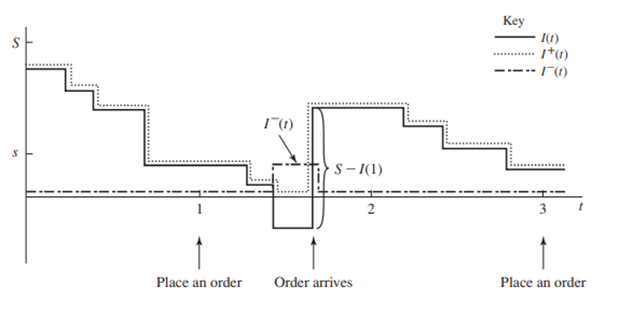
\includegraphics[width=.8\textwidth]{Figures/fig1}
	\caption{تحقق    $I(t)$, $I^+(t)$ و $I^-(t)$}\label{fig1}
\end{figure} 

\newpage
در مدل ما فرض می‌کنیم که شرکت هزینه نگهداری 
$h=1\$$
برای هر آیتم در هر ماه دارد. هزینه نگهداری شامل هزینه هایی مثل اجاره انبار ، بیمه، مالیات و نگهداری می‌باشد.وقتی $I^+(t)=0$ است از هزینه‌های نگهداری صرفنظر می‌کنیم.

به هرحال هدف ما مقایسه سیاست‌های سفارش است صرف‌نظر از این فاکتورکه همه سیاست‌ها مستقل استفاده شده‌اند، تأثیری بر روی تصمیم ما که کدام سیاست بهتراست ندارد. هم اکنون از آن‌جایی که $I^+(t)$ تعداد آیتم‌ها در زمان $t$ را نشان می‌دهد میانگین زمانی در هر ماه برای تعداد آیتم‌هایی که در موجودی برای هر $n$ ماه نگهداری می‌شوند برابراست با: 
\begin{align*}
	\bar{I}^+=\frac{\int_0^n I^+(t)dt}{n}
\end{align*}
که این مقدار شبیه تعریف میانگی زمانی تعداد مشتریان در صف در بخش 1.4.1 می‌باشد. بدین ترتیب میانگین هزینه نگهداری به ازای هر ماه برابر است با $h\bar{I}^+$.

به‌طور مشابه فرض کنید که شرکت هزینه \lr{backlog} برابر با  $\pi=\$ 5$  به ازای هر آیتم در هر ماه در هر مورد در نظر می‌گیرد. که این هزینه اضافی برای مواقعی هست که ما \lr{backlog}
داریم. پس میانگین زمانی تعداد آیتم‌ها در \lr{backlog}
برابراست با:
\begin{align*}
	\bar{I}^-=\frac{\int_0^n I^-(t)dt}{n}
\end{align*}
پس میانگین هزینه \lr{backlog} در هر ماه برابر است با  $\pi\bar{I}^-$.




فرض کنید سطح موجودی اولیه
$I(0)=60 $
باشد و هیچ سفارشی برجسته نباشد.
ما سیستم موجودی را برای
$n=120  $
ماه شبیه سازی می کنیم و از متوسط هزینه کل ماهانه (که حاصل جمع هزینه متوسط سفارش در ماه ، متوسط هزینه نگهداری در ماه و متوسط کمبود هزینه در ماه است) برای مقایسه 9 سیاست موجودی زیر استفاده می کنیم.

$$
\begin{tabular}{llllllllll}
	$s$ & 20 & 20 & 20 & 20 & 40 & 40 & 40 & 60 & 60 \\
	\hline$S$ & 40 & 60 & 80 & 100 & 60 & 80 & 100 & 80 & 100
\end{tabular}
$$
ما در اینجا به این مسئله نمی پردازیم که چگونه این سیاست های خاص برای بررسی انتخاب شده اند. تکنیک های آماری که برای تعیین این سیاست ها مورد استفاده قرار گرفته است در فصل 12 بررسی شده است.
توجه داشته باشید که متغیرهای حالت برای مدل شبیه سازی این سیستم موجودی عبارتند از سطح موجودی
$I(t)$، 
مقدار سفارش برجسته از شرکت به تأمین کننده و زمان آخرین رویداد [که برای محاسبه مناطق تحت توابع
$I^+ (t)$ 
و
$I^- (t)$ 
مورد نیاز است].
\pagebreak

\subsection*{کد \lr{c}}

\label{section:logic}
مدل سیستم موجودی ما از انواع رویداد های زیر استفاده می کند:\\

\begin{center}
	\begin{tabular}{ | m{20em} | m{2cm}| } 
		\hline
		شرح رویداد & نوع رویداد \\ 
		\hline
		دریافت سفارش از طرف تامین کننده به شرکت & 1\\
		\hline
		تقاضای محصول از سمت مشتری & 2 \\
		\hline
		پایان شبیه سازی پس از n ماه & 3 \\
		\hline
		ارزیابی موجودی (و سفارش احتمالی) در ابتدای یک ماه & 4 \\
		\hline
	\end{tabular}
\end{center}
ما تصمیم گرفته ایم که پایان شبیه سازی را رویداد نوع 3 به جای رویداد نوع 4 قرار دهیم، زیرا در زمان 120 رویدادهای "شبیه سازی نهایی" و "ارزیابی موجودی" سرانجام برنامه ریزی می شوند و ما می خواهیم اولین رویداد قبلی را در این زمان اجرا کنیم. (از آنجا که شبیه سازی در زمان 120 به پایان رسیده است ، ارزیابی موجودی و سفارش احتمالی، متحمل شدن هزینه سفارش برای سفارشی که هرگز نخواهد رسید، منطقی نیست). \\
به دلیل اینکه روال زمان بندی در صورت قرار گرفتن همزمان دو یا چند رویداد، رویداد با شماره کوچکتر ترجیح می دهد اجرای رویداد نوع 3 قبل از رویداد نوع 4 تضمین شده است.\\
به طور کلی، برای پردازش وقایعی که در ترتیب مناسب هنگام وقوع پیوندهای زمانی رخ می دهند باید یک مدل شبیه سازی طراحی شود.
نمودار رویداد (به بخش 1.4.7 مراجعه کنید) در شکل 2 ظاهر می شود.
\\

سه نوع متغیر تصادفی برای شبیه سازی این سیستم وجود دارد. زمان های میان تقاضا به صورت نمایی توزیع شده اند بنابراین از همان الگوریتم (و کد) که در بخش 1.4 توسعه یافته است، در اینجا می توان استفاده کرد. متغیر تصادفی میزان تقاضا
$D$
باید گسسته باشد، همانطور که در بالا توضیح داده شد، و می تواند به صورت زیر تولید شود. ابتدا فاصله واحد را به زیر فواصل مجاور

$\cdot C_{4}=\left[\frac{5}{6}, 1\right) \cdot C_{3}=\left[\frac{1}{2}, \frac{5}{6}\right) \cdot C_{2}=\left[\frac{1}{6}, \frac{1}{2}\right) \cdot C_{1}=\left[0, \frac{1}{6}\right)$

تقسیم می کنیم و یک توزیع یکنواخت تصادفی
$ U(0,1) $
که متغییر تصادفی
$ U $
است از یک تولید کننده عدد رندوم بدست می آید.

\begin{center}
	\begin{figure}[hpt]
		\centering
		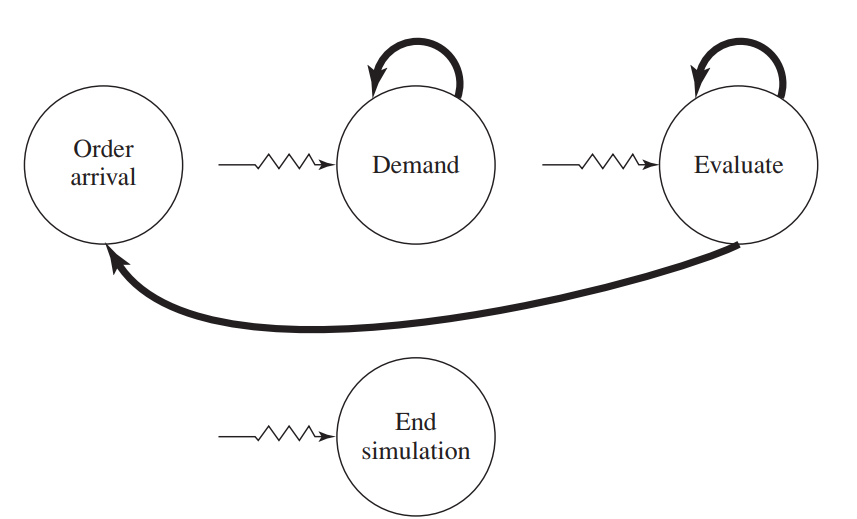
\includegraphics[width=1\textwidth]{Figures/29.png}\hfill
		\caption{گراف رویداد، مدل \lr{inventory} }
		\label{شکل 29}
	\end{figure}
\end{center}

اگر \lr{U} در \lr{c1} قرار گرفت، $D = 1 $ را برمیگرداند. اگر \lr{U}   در \lr{c2} قرار گرفت، $ D=2 $رابرمیگرداند و به همین ترتیب. از آنجا که عرض \lr{c1} برابر با 
$\dfrac{1}{6}-0 = \dfrac{1}{6}$ 
است، احتمال اینکه \lr{U} در \lr{c1} قرار بگیرد (و$ D=5 $را برگرداند)  برابر با $\dfrac{1}{6}$   است. این با احتمال دلخواه $ D=1 $ مطابقت دارد. به طور مشابه، اگر \lr{U} در \lr{c2} قرار بگیرد،$ D=2 $ را برمیگردانیم و طبق احتمال، برابر با عرض \lr{c2} یعنی 
$\dfrac{1}{2}-\dfrac{1}{6} = \dfrac{1}{3}$
است. به همین ترتیب برابر فواصل دیگر.  زیر برنامه برای تولید اندازه درخواست از این اصل استفاده می کند و نقاط برش تعریف شده بالا فاصله ی فرعی که احتمال تجمعی توزیع \lr{D} است را به عنوان ورودی می گیرد.

تاخیر های تحویل به طور یکنواخت توزیع می شوند، اما روی فاصله ی واحد $[0,1] $ نیستند. به طور کلی می توانیم با تولید یک عدد تصادفی \lr{U }با توزیع \lr{uniform} $(0,1)$ و سپس بازگرداندن$ a+U(b-a)$ یک متغییر تصادفی توزیع شده به صورت یکنواخت در هر بازه ی $[a,b] $ تولید کنیم. صحیح بودن این روش به صورت شهودی واضح است، اما به طور رسمی در بخش $Sec 8.3.1 $ توجیه خواهد شد.

اکنون ما منطق انواع رخداد $ 1,2 $و $4 $ را توصیف می کنیم که در واقع شامل تغییرات حالت است.

فلوچارت رویداد ورود سفارش در شکل\ref{fig:order-arrival} نمایش داده می شود. باید تغییرات لازم هنگام ورود سفارش( که قبلا انجام شده بود) از تامین کننده انجام شود. سطح موجودی کالا (\lr{inventory level}) با افزایش مقدار سفارش افزایش می یابد و رویداد ورود سفارش باید از منظر بررسی حذف شود. (برای بررسی این مسئله که آیا می توان همزمان بیش از یک سفارش برای این مدل با این پارامترها داشت ، به شماره$ 1.12$ مراجعه کنید.)

یک فلوچارت برای رویداد درخواست(\lr{demand}) در شکل \ref{fig:demand}  آورده شده است و تغییرات لازم برای نشان دادن وقوع درخواست را پردازش می کند. ابتدا اندازه درخواست تولید می شود و \lr{inventory} به وسیله ی این مقدار کاهش می یابد. سرانجام، زمان درخواست بعدی در لیست رویداد برنامه ریزی می شود. توجه داشته باشید که این مکانی است که ممکن است \lr{inventory level } منفی شود.

پیشامد ارزیابی موجودی، که در ابتدای هر ماه اتفاق می افتد، در تصویر \ref{fig:evaluate} نشان داده شده است. اگر سطح موجودی $I(t)$ در زمان ارزیابی حداقل $s$ باشد، هیچ سفارشی انجام نمی‌شود و هیچ کاری انجام نمی‌شود مگر برای زمان‌بندی ارزیابی بعدی در لیست پیشامدها. از طرف دیگر، اگر $I(t) < s$ باشد، می‌خواهیم برای اقلام $S - I(t)$ سفارش بدهیم. این کار با ذخیره مقدار سفارش $[S - I(t)]$ تا رسیدن سفارش و زمان‌بندی زمان رسیدن آن انجام می‌شود. در این مورد نیز می خواهیم پیشامد ارزیابی موجودی بعدی را زمان‌بندی کنیم.\\
همانطور که در مدل صف‌بندی تک سرور است، نوشتن یک روال بدون پیشامد جداگانه برای به روزرسانی انباشتگران آماری زمان پیوسته، راحت است. با این حال، برای این مدل، انجام این کار کمی پیچیده‌تر است، بنابراین ما یک نمودار برای این فعالیت در شکل \ref{fig:update-time-avg-stats} ارائه می‌دهیم. مسئله اصلی این است که آیا ما باید منطقه تحت $I^{-}(t)$ یا $I^{+}(t)$ را به روز کنیم (یا هیچ کدام). اگر سطح موجودی از آخرین پیشامد منفی بوده است ، پس ما در لیست عقب مانده هستیم، بنابراین فقط منطقه تحت $I^{-}(t)$ باید به روز شود. از طرف دیگر، اگر سطح موجودی مثبت بوده است، فقط باید سطح زیر $I^{+}(t)$ را به روز کنیم. اگر سطح موجودی صفر بوده باشد (یک احتمال وجود دارد)، هیچ یک از به روزرسانی‌ها لازم نیست. کد این روال همچنین متغیر مربوط به زمان آخرین پیشامد را به زمان حال می‌رساند. صرف نظر از نوع پیشامد یا اینکه واقعاً سطح موجودی در این نقطه در حال تغییر است، این روال، درست پس از بازگشت از روال زمان‌سنجی از برنامه اصلی فراخوانی می‌شود. این، یک روش ساده (اگر نه کارآمدترین از نظر محاسباتی) از بروزرسانی انتگرال‌ها برای آمار زمان پیوسته را فراهم می‌کند.
\begin{figure}[h]
\centering
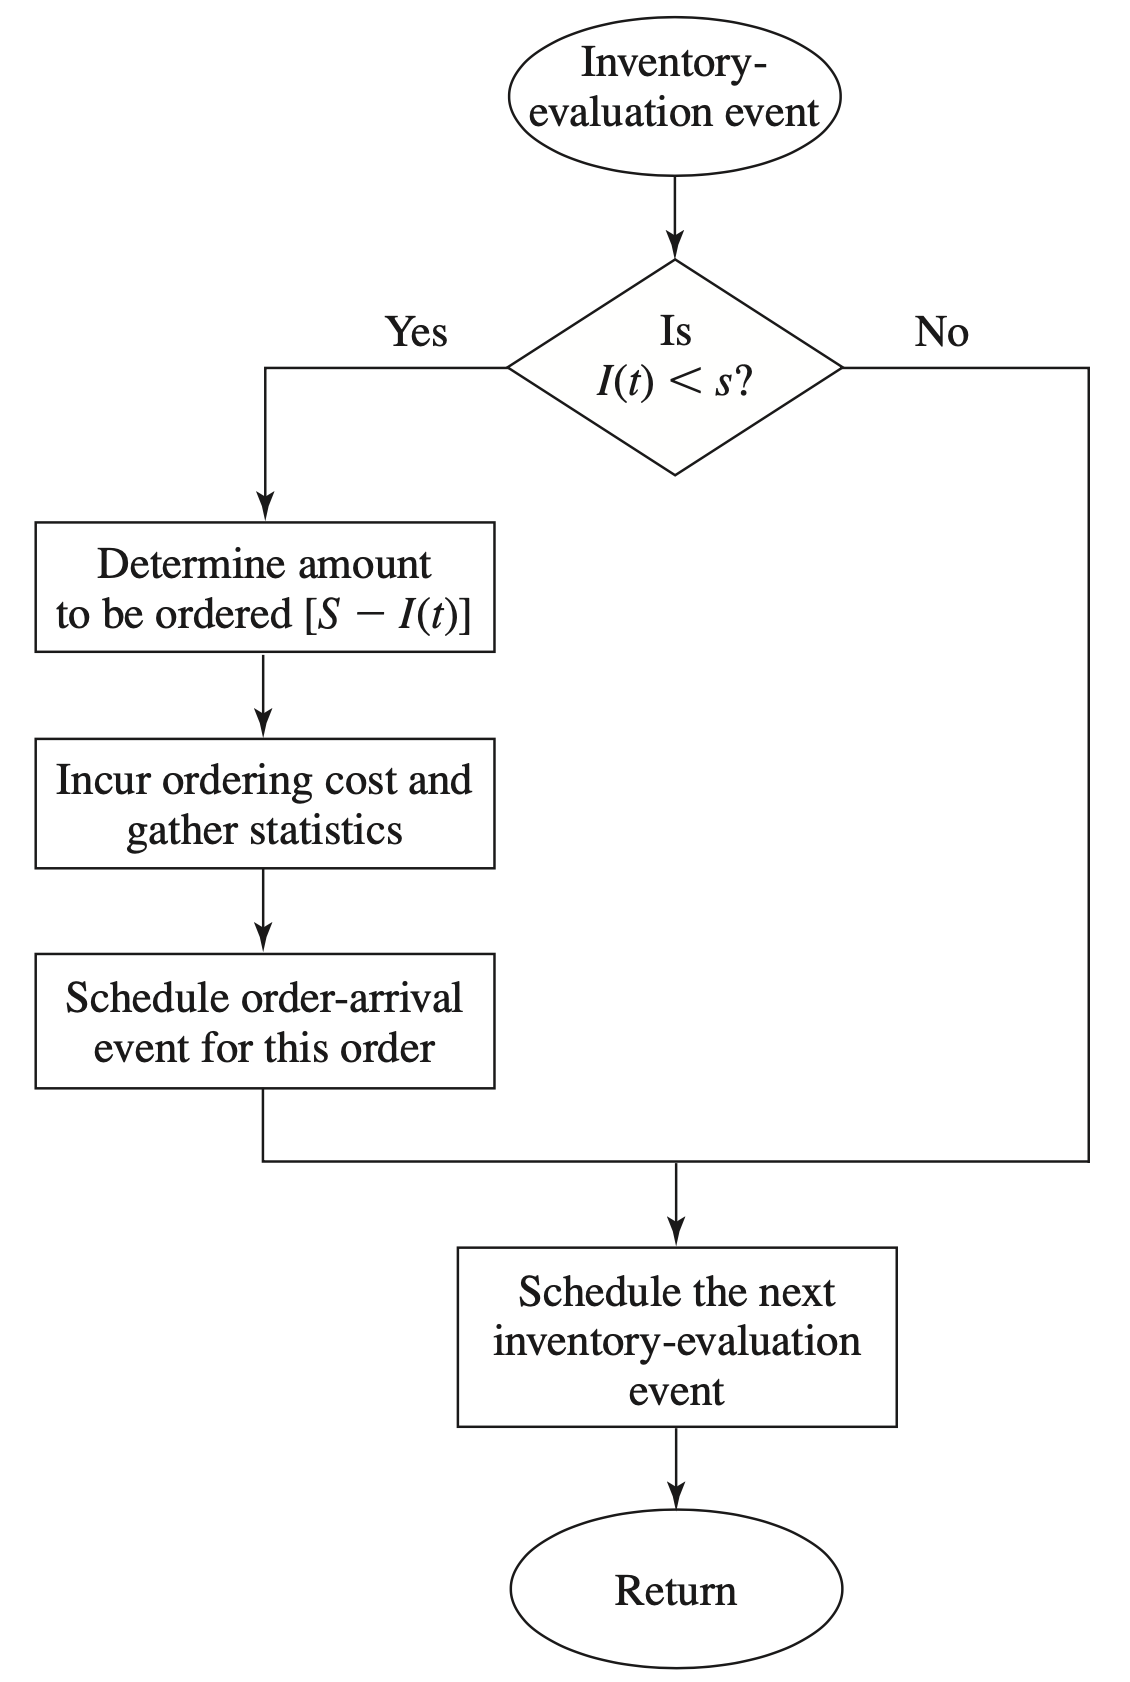
\includegraphics[width=0.40\textwidth]{Figures/evaluate.png}
\caption{نمودار روال ارزیابی موجودی، مدل موجودی.}
\label{fig:evaluate}
\end{figure}

بخش \ref{section:c-program} حاوی برنامه‌ای برای شبیه‌سازی این مدل در \lr{C} است. هیچکدام از زیربرنامه‌های زمان‌سنجی و یا تولید متغیر نمایی نمایش داده نخواهند شد، زیرا همانند مدل صف‌بندی تک سرور در بخش ۱.۴ هستند. خواننده همچنین باید شباهت قابل توجه بین برنامه های اصلی صف‌بندی و مدل‌های موجودی را ذکر کند.

\pagebreak

\subsection*{\lr{MATLAB Code}}

کد های متلب را میتوانید در فایل مربوطه ببینید، در اینجا صرفا خروجی را نشان میدهیم:


	\begin{figure}[hpt]
		\centering
		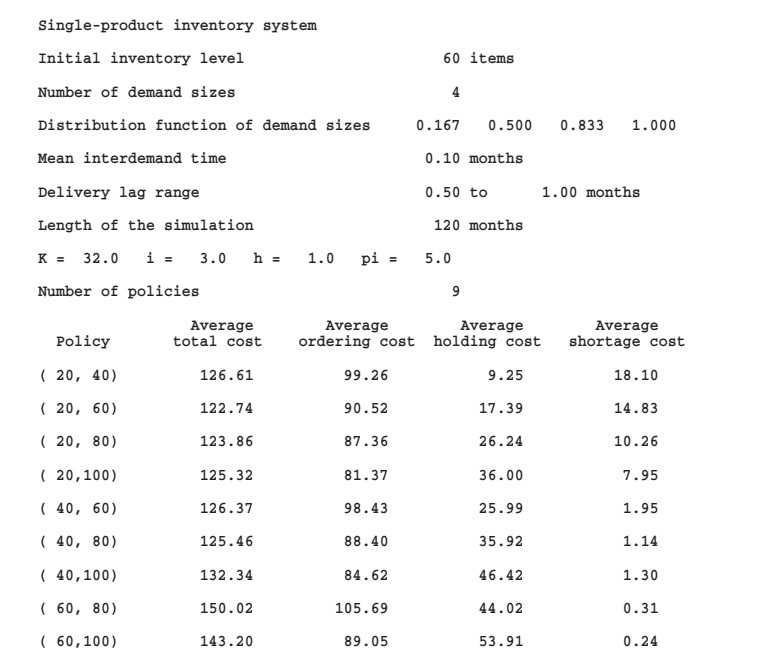
\includegraphics[width=1\textwidth]{Figures/MM}
	\end{figure}

که متشابه هستند
	
\end{document}